\subsection{Inclusive Selection: Hadronic channel}
\label{subsec:sel_incl_hadronic}
%\textcolor{red}{To be updated from Phys14 to Spring15 studies before full stats}
Events for the hadronic channel are obtained with two triggers. For events from runs before 254227, the trigger used is HLT\_PFMET170\_NoiseCleaned\_PFMHTNoMu120\_IDTight, while for subsequent runs, the trigger is HLT\_PFMETNoMu120\_JetIdCleaned\_PFMHTNoMu120\_IDTight. The efficiency of these triggers with respect to offline $\met$ in the single electron and single muon channels is shown in Fig.~\ref{fig:meteff_0}. Discrepancies in the turn-on curves between the two channels are under investigation. Overall efficiencies at the plateau in both channels are in agreement between data and MC (comparing the fit parameter $\epsilon_{0}$ and the fit).This dictates the use of a unity scale factor for data-to-MC $\met$ corrections.

\begin{figure}[htbp]
\centering
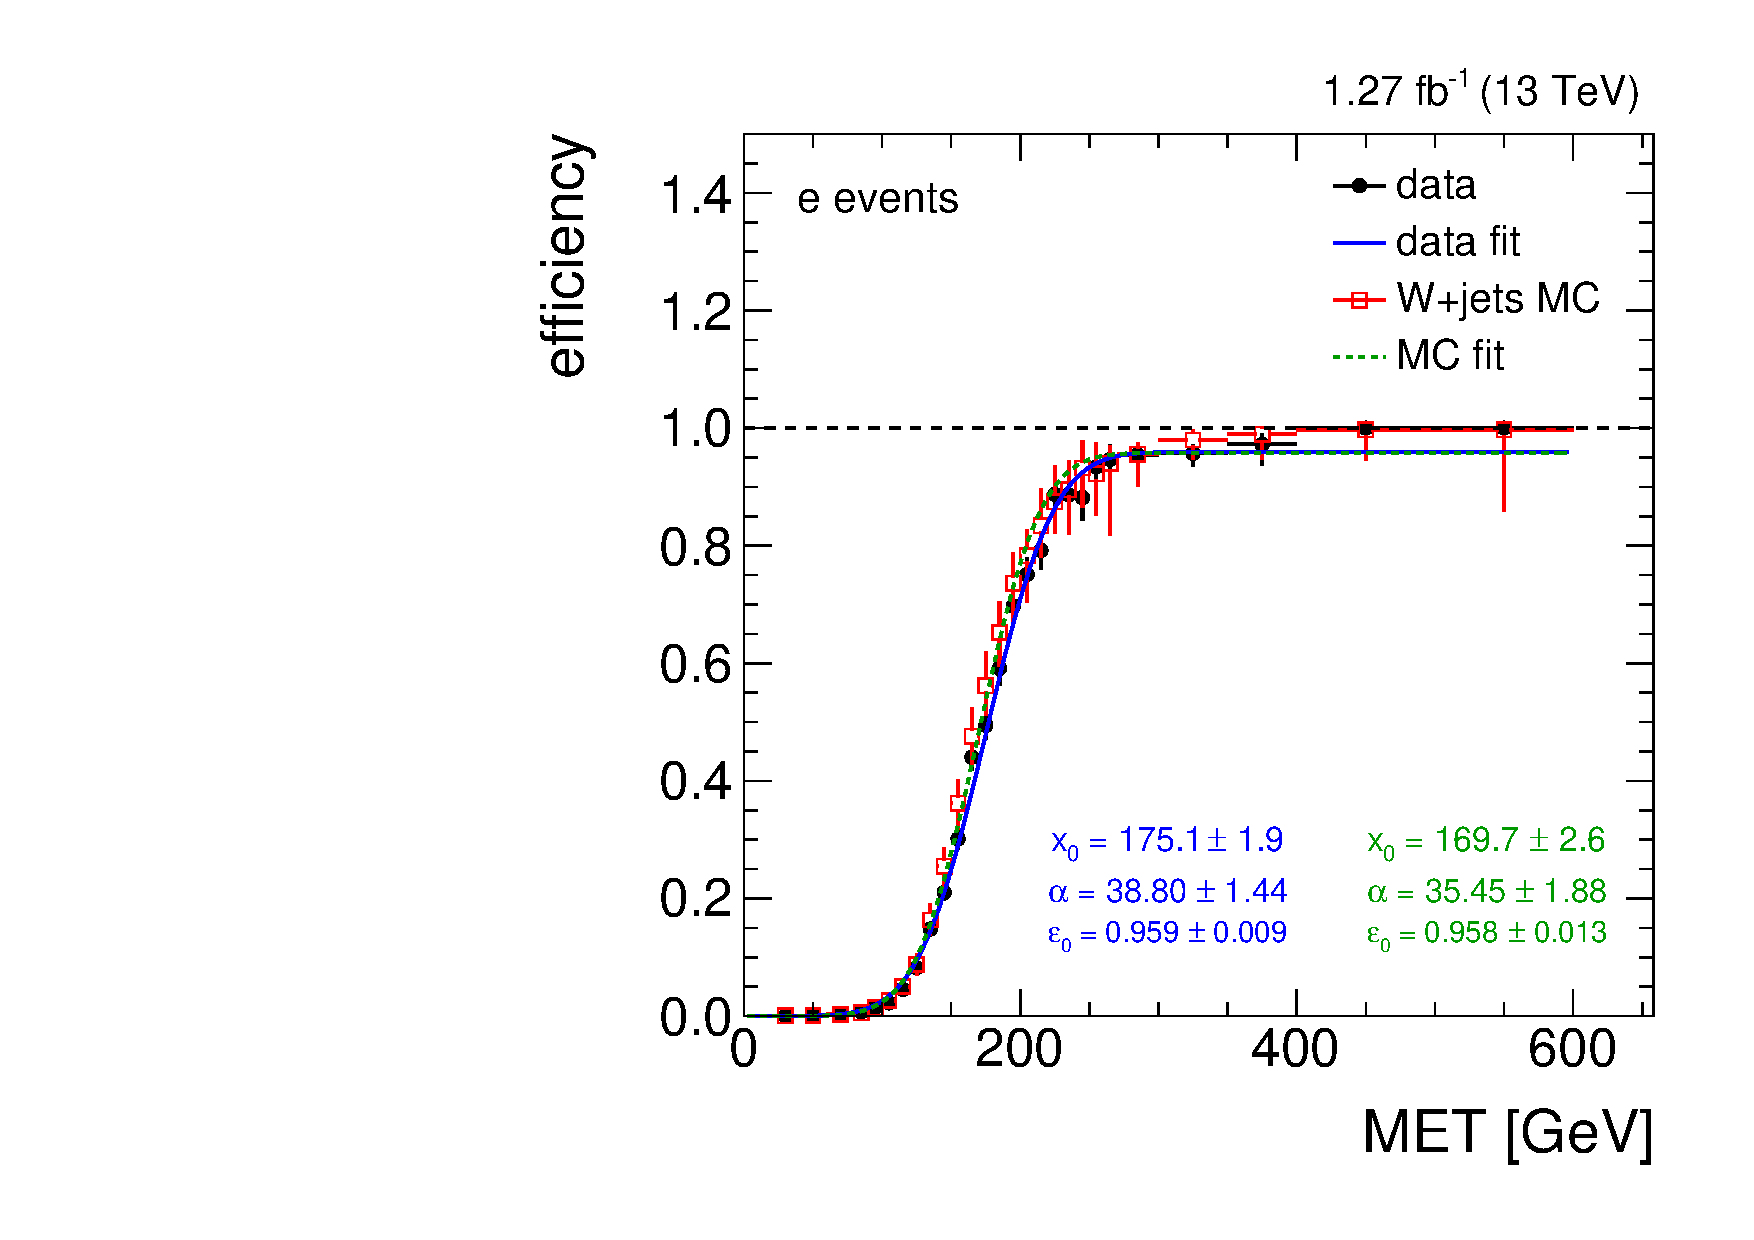
\includegraphics[width=0.48\textwidth]{figures/meteff_e_1.pdf}
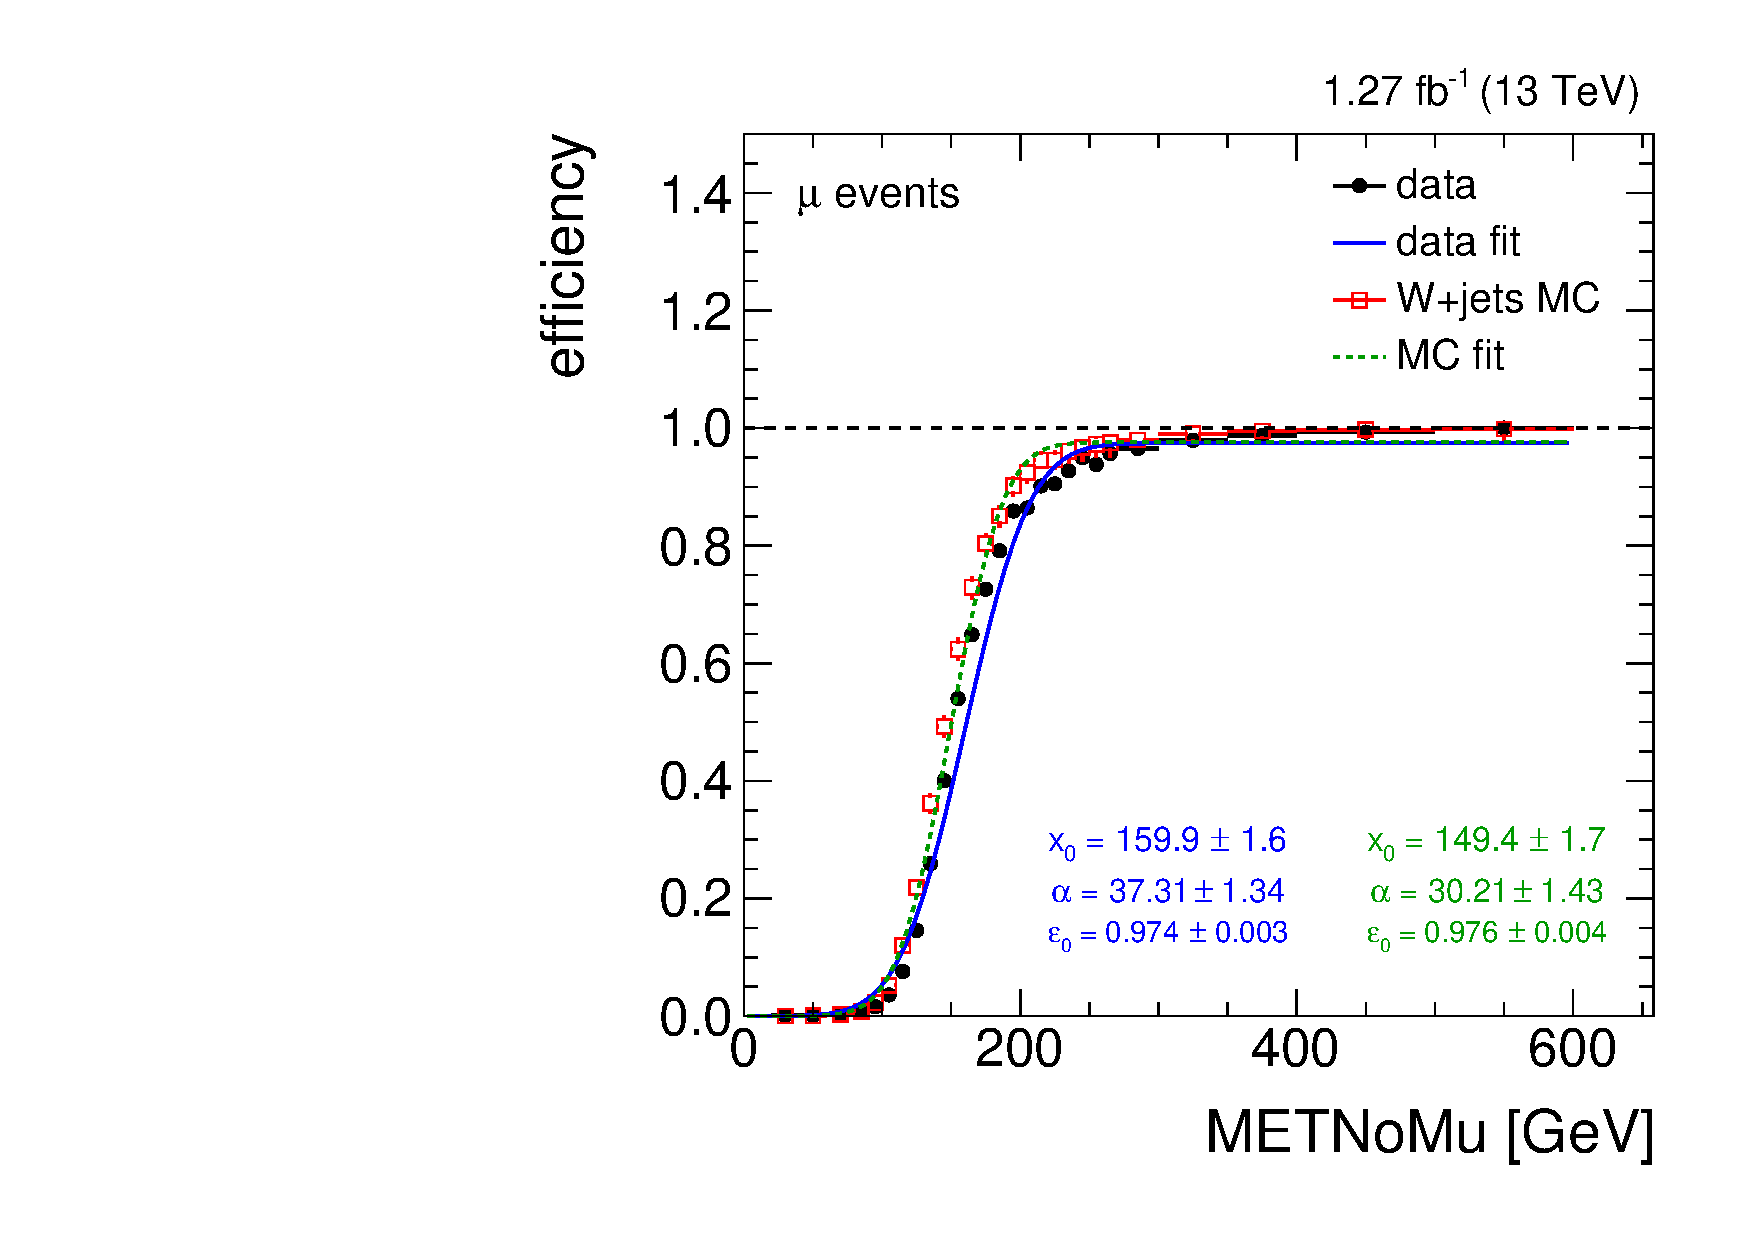
\includegraphics[width=0.48\textwidth]{figures/meteff_m_1.pdf}
\caption{Efficiency turn-on curves of HLT\_PFMET170\_NoiseCleaned\_PFMHTNoMu120\_IDTight and HLT\_PFMETNoMu120\_JetIdCleaned\_PFMHTNoMu120\_IDTight for electron events (left) and muon events (right). Events are required to have at least four jets.}
\label{fig:meteff_0}
\end{figure}

\begin{figure}[htbp]
  \centering
  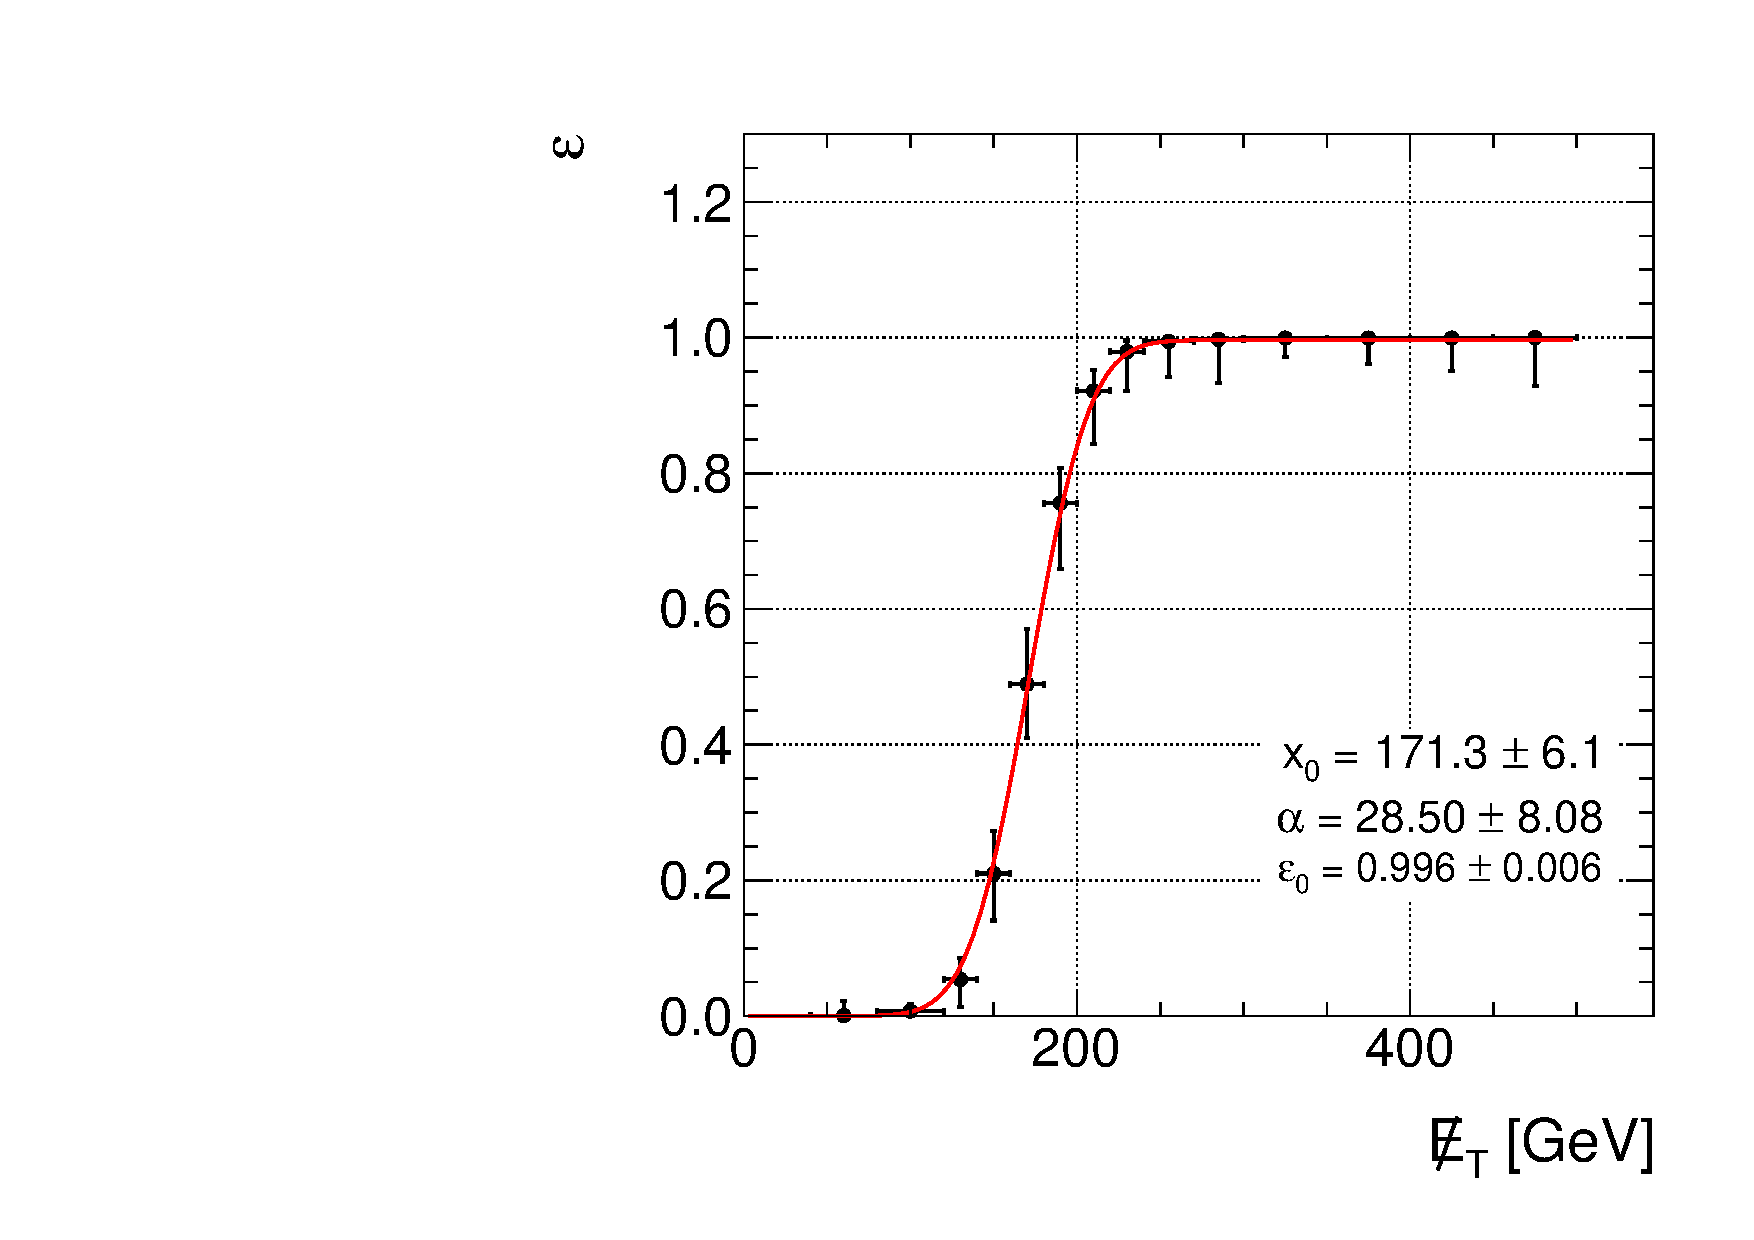
\includegraphics[width=0.48\textwidth]{figures/ttdm1-meteff.pdf}
  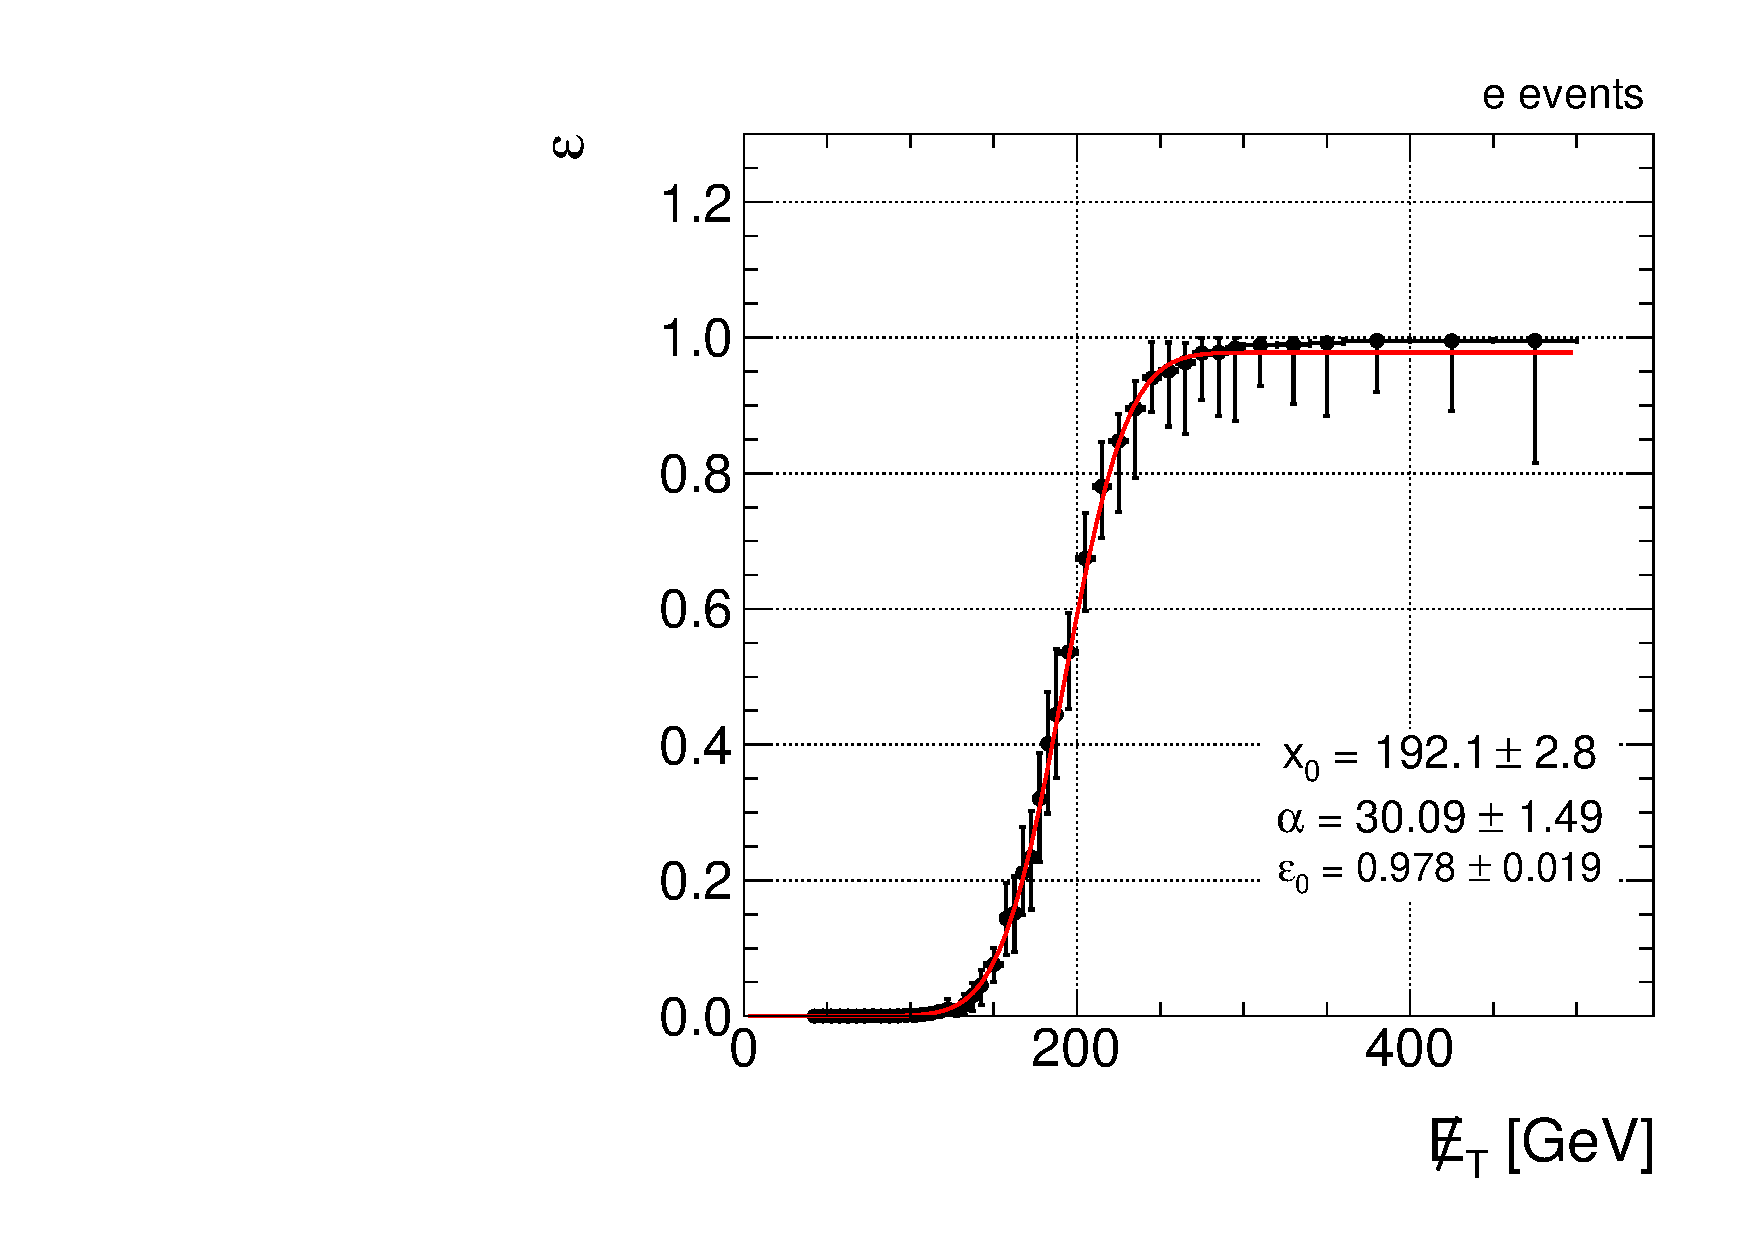
\includegraphics[width=0.48\textwidth]{figures/wjets-e-meteff.pdf}
  \caption{Efficiency turn-on curves of HLT\_PFMET170\_NoiseCleaned for $\ttbar+$DM EFT signal with $M_{\chi}=1$ (left), and for electron events in $\Wjets$ passing a single electron trigger (right). Events are required to have at least four jets.}
  \label{fig:meteff_1}
\end{figure}

The offline event selection requires,
\begin{itemize}
\item $\met > 250\:\GeV$, to be on the plateau of the efficiency turn-on curve,
\item at least $4$ AK4CHS jets with $\pt>30\:\GeV$ and $|\eta|<4$,
  \begin{itemize}
  \item at least $2$ of which have $|\eta|<2.4$ and $\Bot$-tagged,
  \end{itemize}
\item no muons passing ``Loose'' selection with $\pt>10\:\GeV$ and $|\eta|<2.4$,
\item no electrons passing ``Veto'' selection with $\pt>10\:\GeV$ and $|\eta|<2.5$,
\item $\min_{i=1,\ldots,6}\Delta\phi\left(j_i,\met\right)>1$, the minimum $\Delta\phi$ between jet and $\met$ considering up to the sixth leading jet.
\end{itemize}

The $\min_{i=1,\ldots,6}\Delta\phi\left(j_i,\met\right)$ distribution after all other selection cuts is shown in Fig.~\ref{fig:dphijetmet6}. The cut on this variable reduces the QCD multi-jets background to negligible levels. It also reduces the $\ttbar$ background, which is predominantly semileptonic.%, because events with high $\met$ have a boosted $\Top$ quark and therefore the neutrino and $\Bot$ jet will be close to each other. 
It was studied that considering $\Delta\phi$ for up to the sixth leading jet performs better than considering fewer number of jets and better than considering all jets. These studies are presented in Appendix~\ref{app:dphijetmet}.

\begin{figure}[htbp]
  \centering
  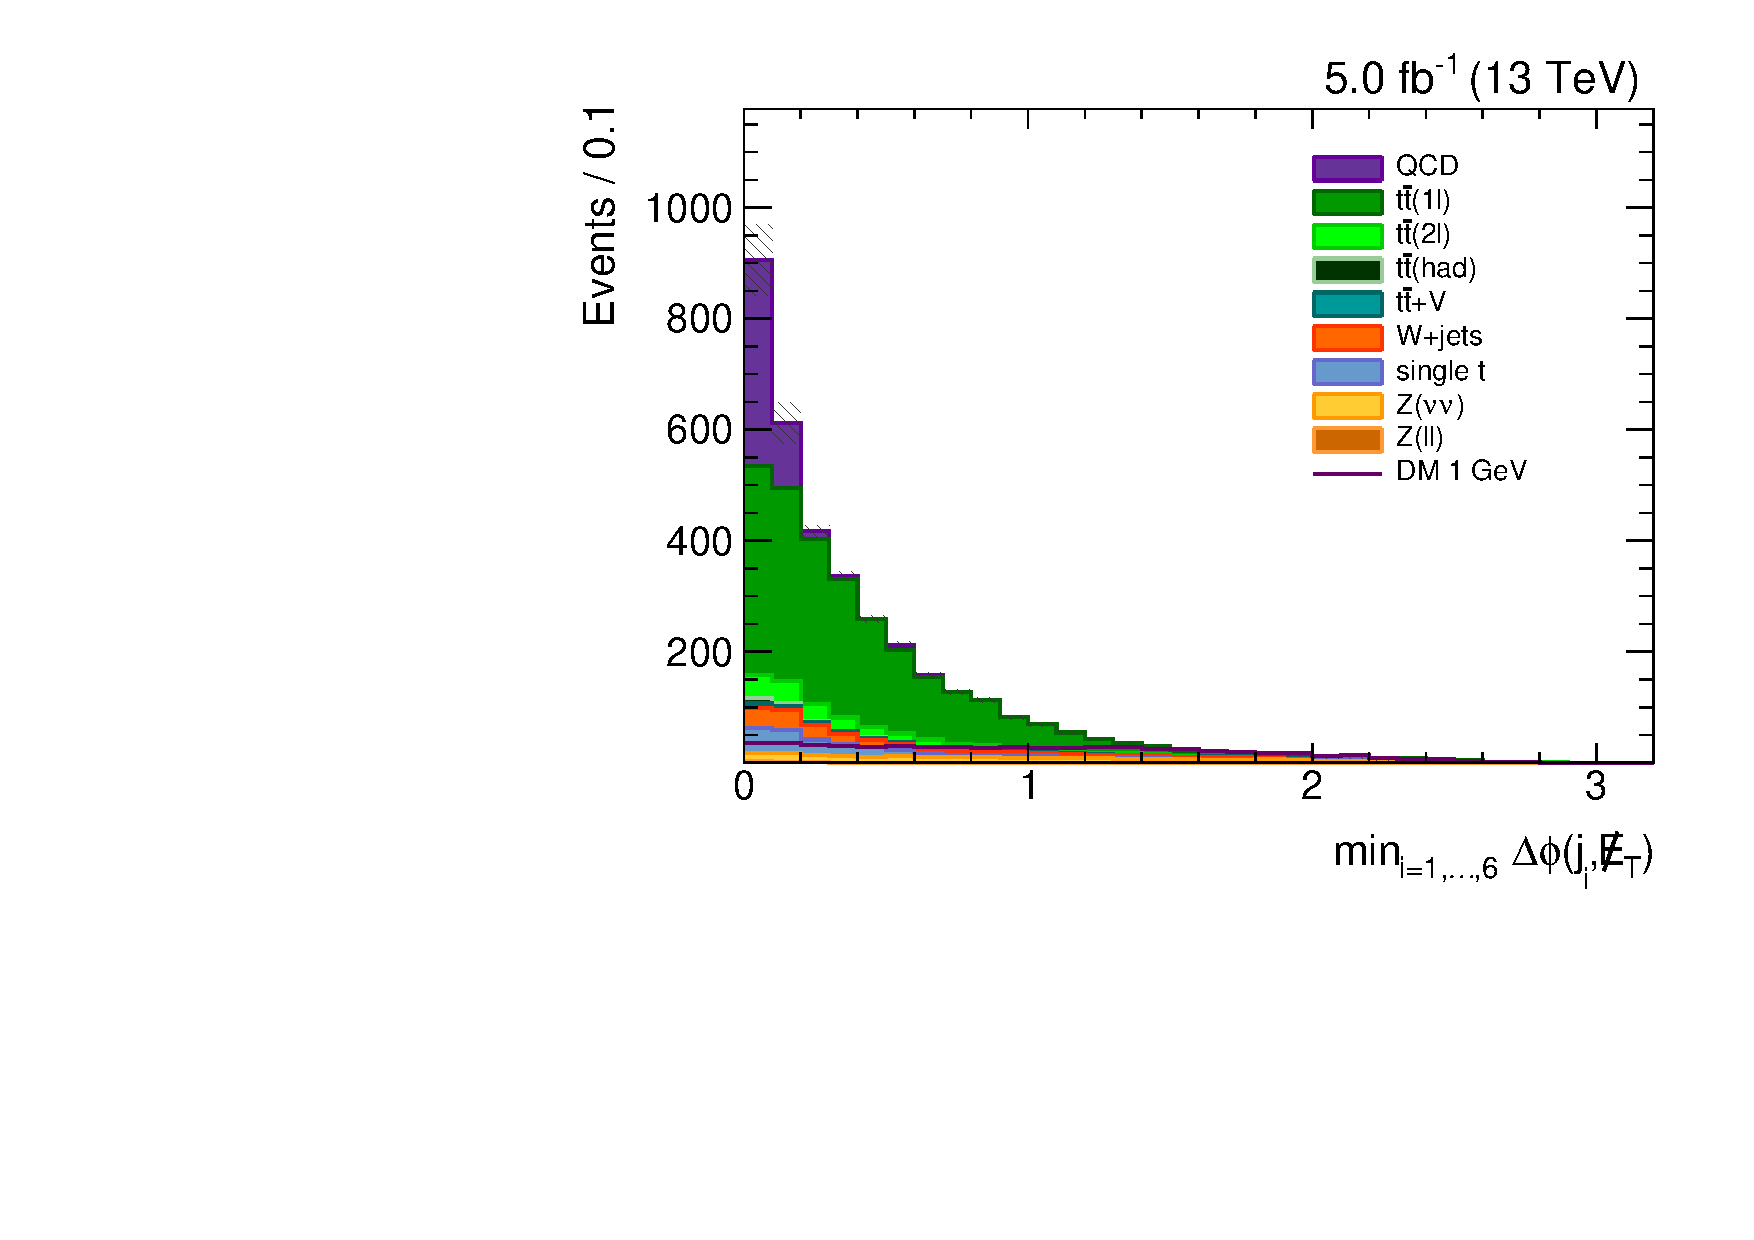
\includegraphics[width=0.48\textwidth]{figures/hadronic-incl-dphijetmet6.pdf}
  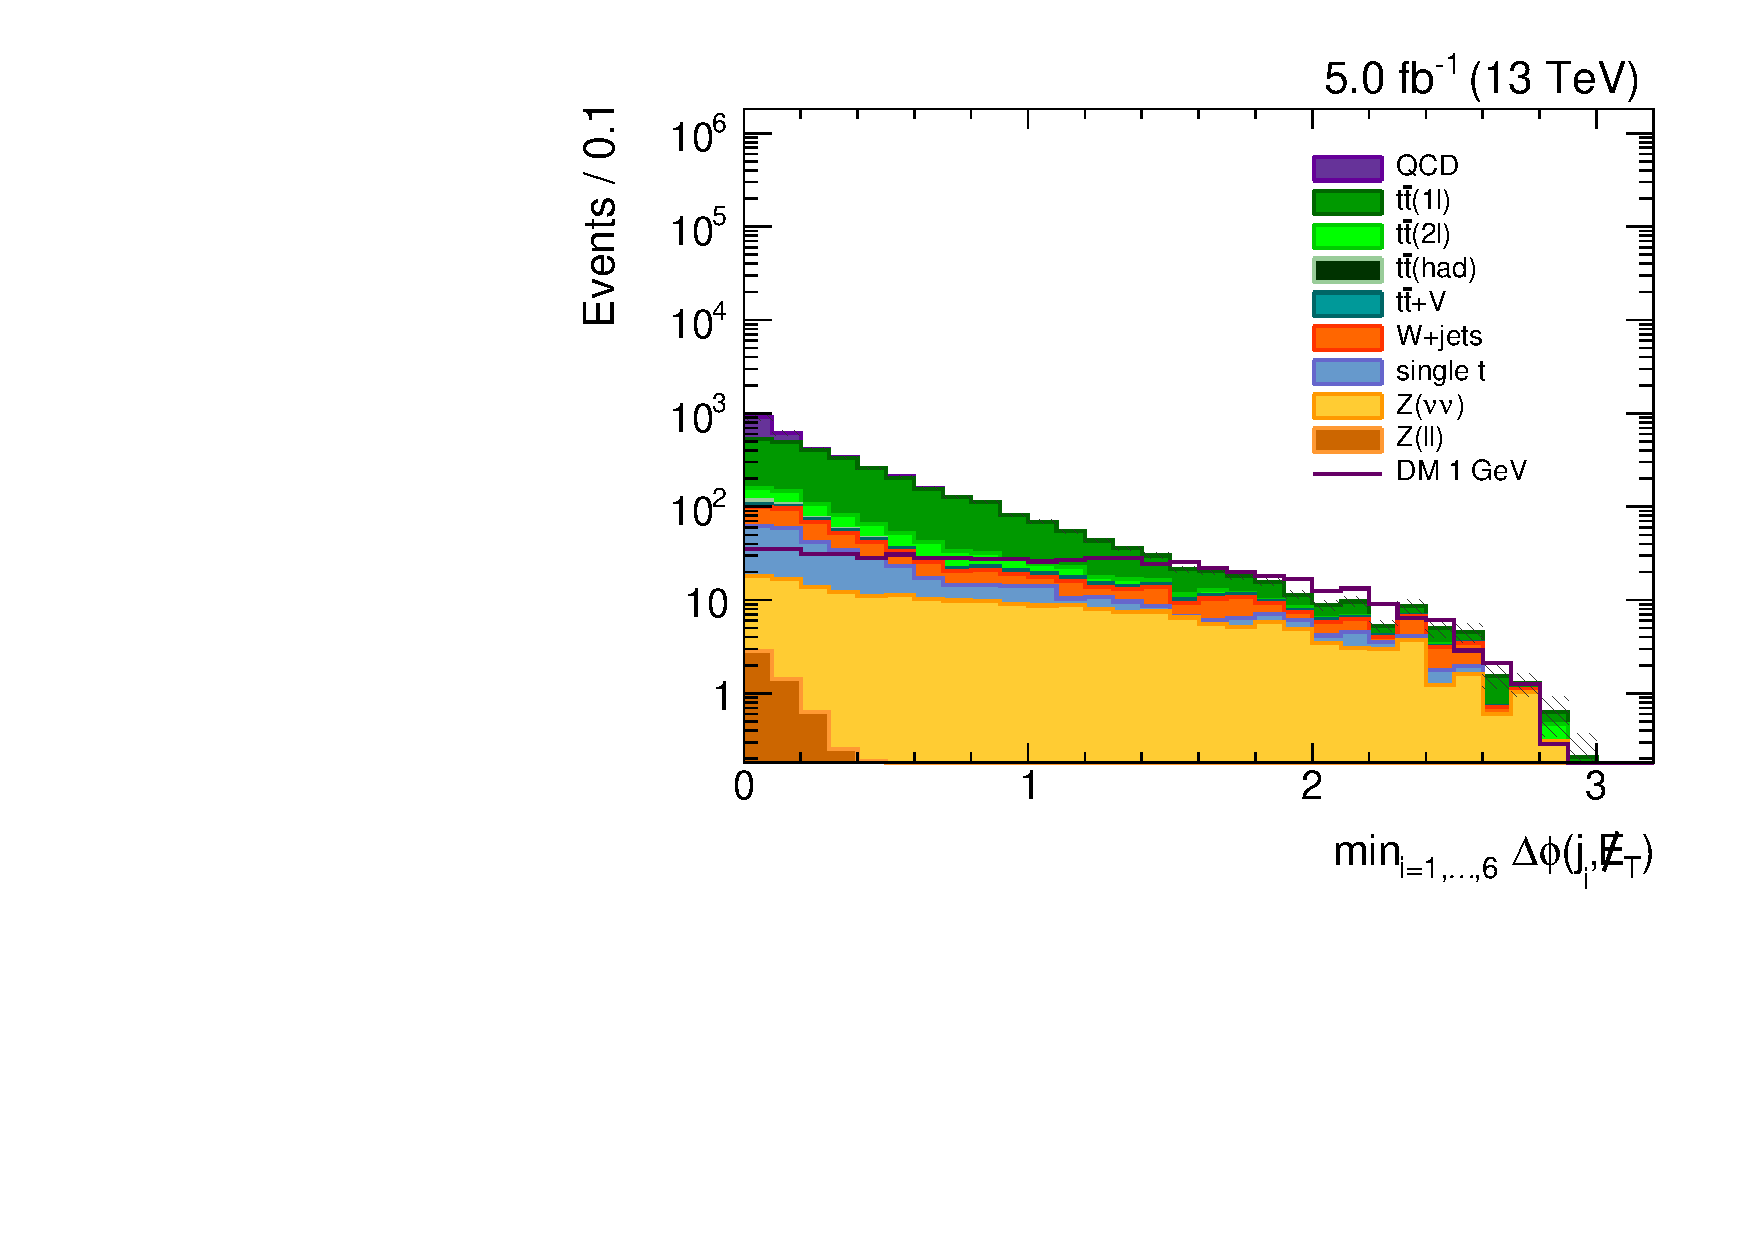
\includegraphics[width=0.48\textwidth]{figures/hadronic-incl-dphijetmet6log.pdf}
  \caption{The $\min_{i=1,\ldots,6}\Delta\phi\left(j_i,\met\right)$ distribution in linear scale (left) and log scale (right).}
  \label{fig:dphijetmet6}
\end{figure}

The $\met$ distributions before and after cutting on $\min_{i=1,\ldots,6}\Delta\phi\left(j_i,\met\right)$ are shown in Fig.~\ref{fig:incl_hadronic_met}. The expected yields for $5\:\ifb$ after selection are shown in Table~\ref{tab:incl_hadronic_yields}.

\begin{figure}[htbp]
  \centering
  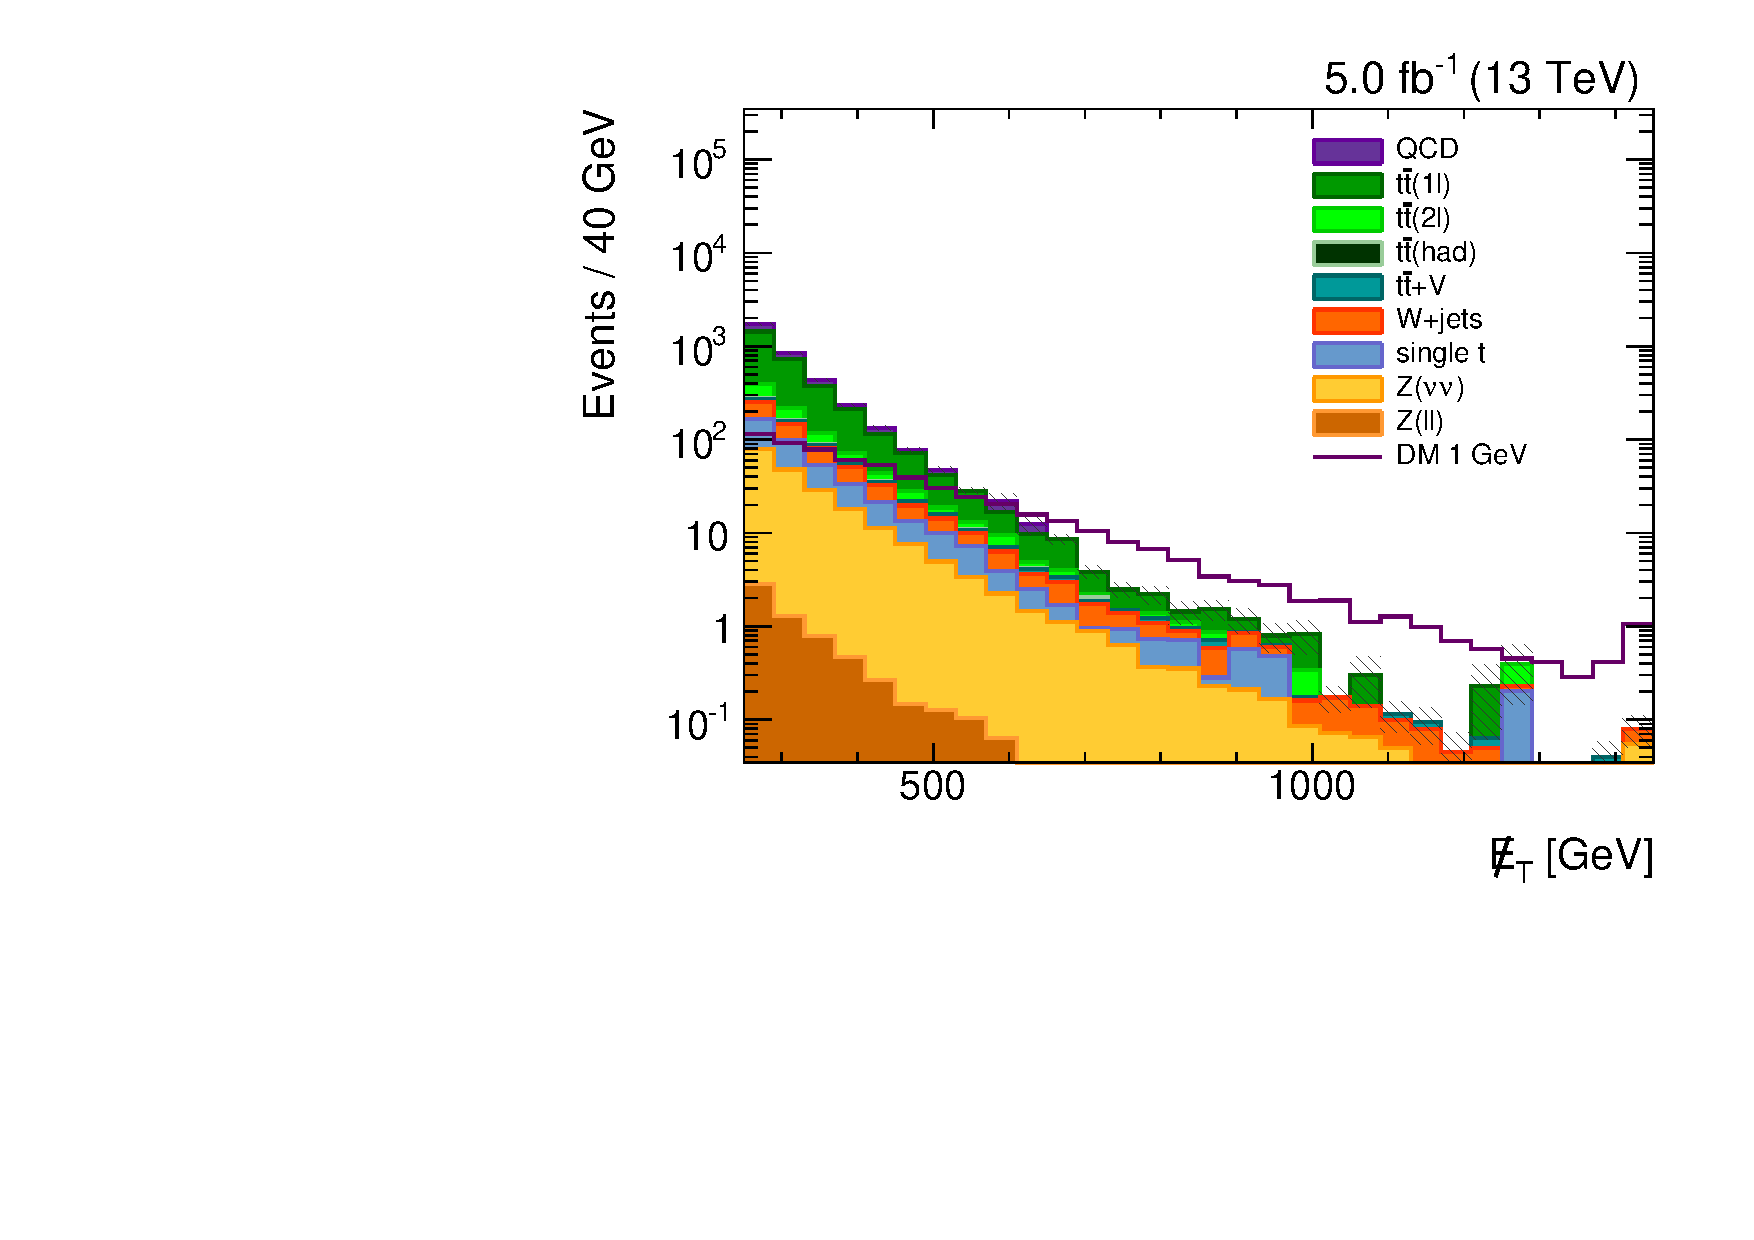
\includegraphics[width=0.48\textwidth]{figures/hadronic-incl-metlog_nodphi.pdf}
  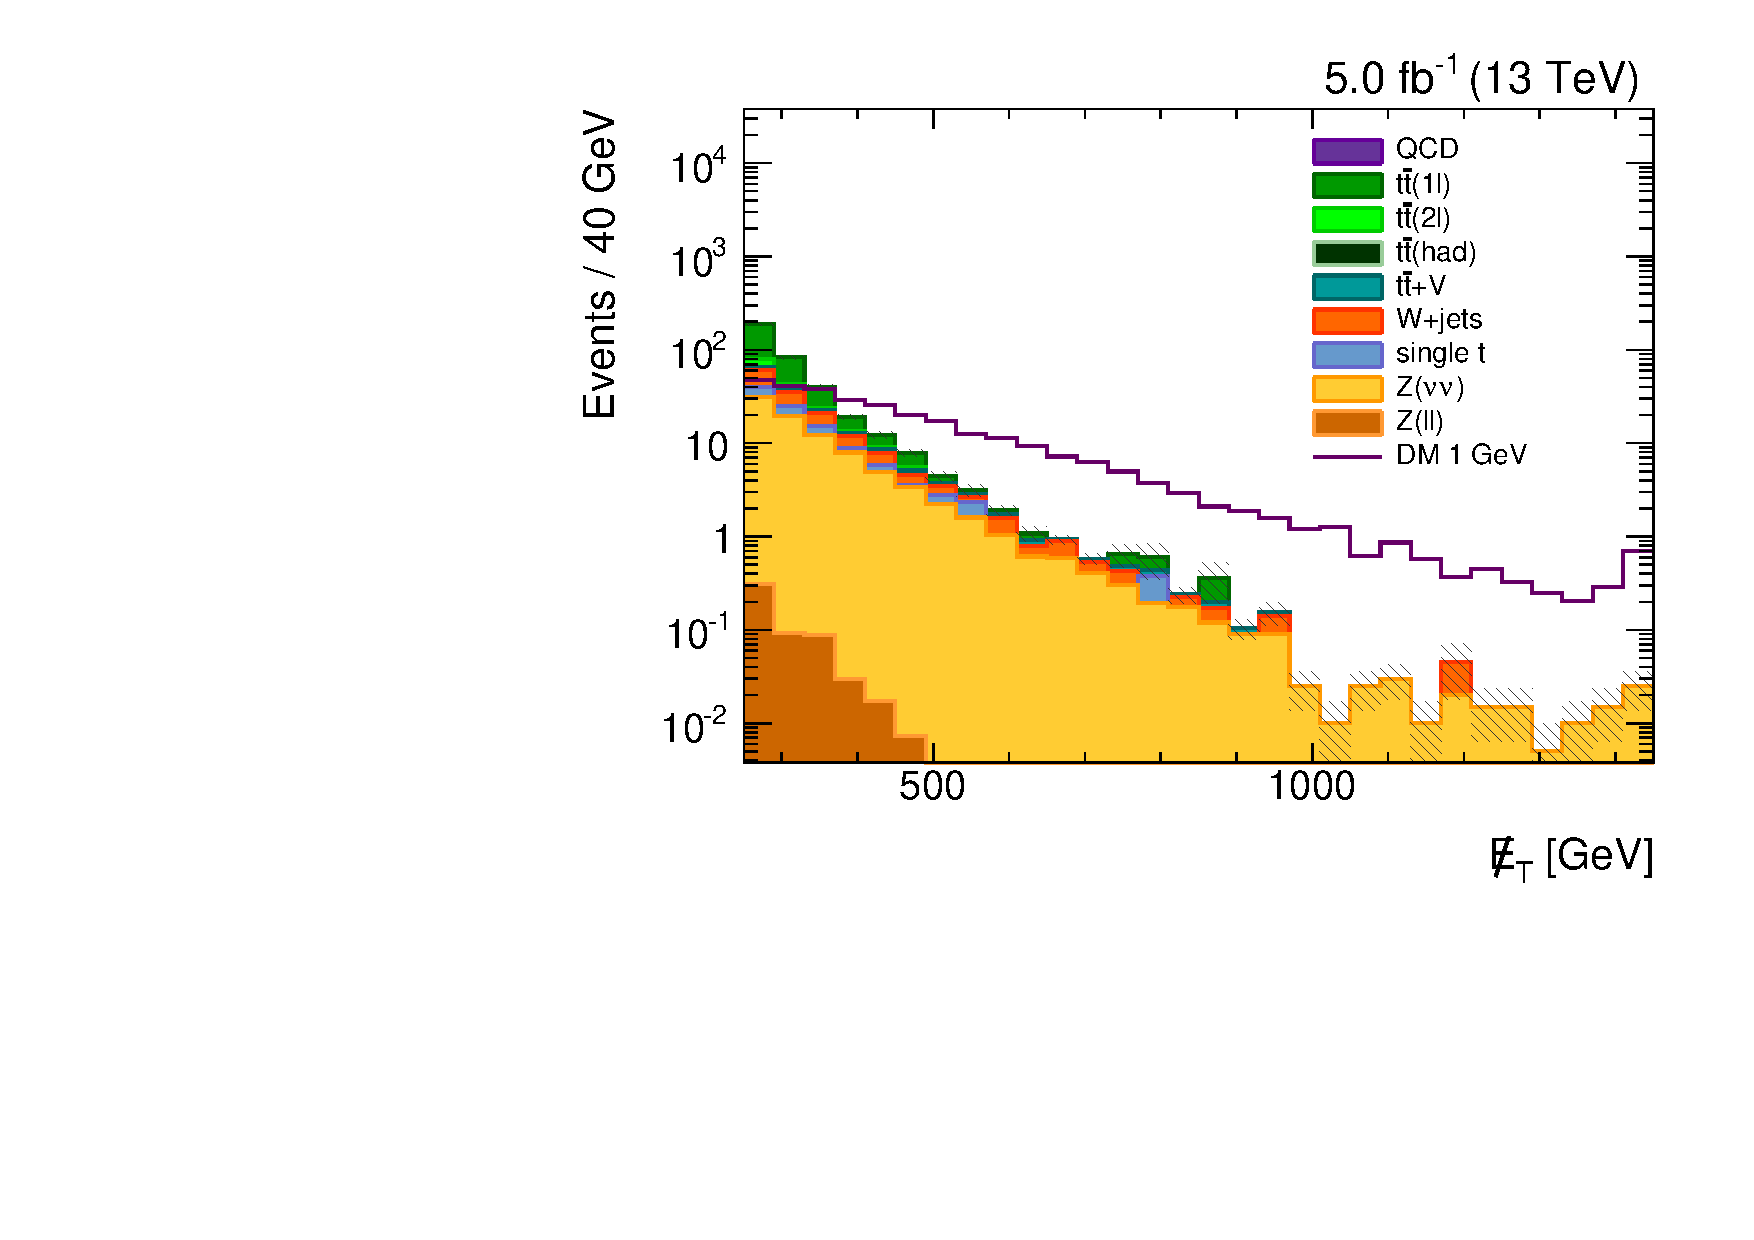
\includegraphics[width=0.48\textwidth]{figures/hadronic-incl-metlog.pdf}
  \caption{The $\met$ distribution before (left) and after (right) the cut on $\min_{i=1,\ldots,6}\Delta\phi\left(j_i,\met\right)$. Note that the right-most bin includes overflow.}
  \label{fig:incl_hadronic_met}
\end{figure}

\begin{table}[!ht]
\centering
\begin{tabular}{|c|r|}
\hline
  Process               & \multicolumn{1}{|c|}{Yields} \\
\hline
  \Z\To\Lep\Lep         & $  0.54 \pm 0.12$ \\
  \Z\To\Nu\Nu           & $ 86.09 \pm 1.82$ \\
  Single \Top           & $ 21.36 \pm 1.89$ \\
  \Wjets                & $ 45.42 \pm 3.11$ \\
  QCD                   & $  0.00 \pm 0.00$ \\
  $\ttbar+V$            & $ 11.19 \pm 0.40$ \\
  $\ttbar(\mbox{had})$  & $  0.00 \pm 0.00$ \\
  $\ttbar(1\Lep)$       & $179.61 \pm 5.42$ \\
  $\ttbar(2\Lep)$       & $ 21.74 \pm 1.88$ \\
\hline
  SM expected           & $365.94 \pm 7.04$ \\
\hline
  $M_\chi=1\:\GeV$      & $289.61 \pm 3.45$ \\
\hline
\end{tabular}
\caption{Expected yields for $5\:\ifb$ after the inclusive selection for the hadronic channel.}
\label{tab:incl_hadronic_yields}
\end{table}
